%!TEX root = ../report.tex

\chapter{Results}

Since the major contribution of this work is the creation of the dataset, the experiments are focussed on validating the effectiveness of the dataset. 

% Add visual segmentation masks in all results.

\subsection{Results on the complete validation set}

% both variety of backgrounds and white backgrounds

Deeplabv3+ with both the mobileNet backbone and the xception backbone are evaluated on all variants of variety of backgrounds and white backgrounds dataset. From \ref{Fig:mobivars}, it is evident that the Mean IOU obtained on each variant is dependent on the properties of objects in the variant. The atWork\_full variant treats all the 18 objects in the dataset as different classes. As a result, for instance, m20 and m30 have different labels despite the fact that the two objects only differ in size and slightly in color. The segmentation model is thus forced to distinguish between such objects. Since the objects occur in the dataset in arbitrary scales and are subject to differences in illumination, the real world differences between such similar objects become insignificant in the dataset. Thus, the Mean IOU obtained in the atWork\_full variant is indeed the lowest as expected. The two variants atWork\_size\_invariant and atWork\_similar\_shapes combine objects which are similar. As a result, the segmentation model achives better Mean IOU on these variants. The atWork\_binary variant requries the segmentation model to only distinguish foreground from background leading to the highest MIOU. From \ref{Fig:xcepvars}, deepLabV3+ with the xception backbone, evidently, also follows a similar trend like deepLabv3+ with mobileNet backbone.

	\begin{figure}[!htb]
		\begin{subfigure}{.5\textwidth}
			\centering
			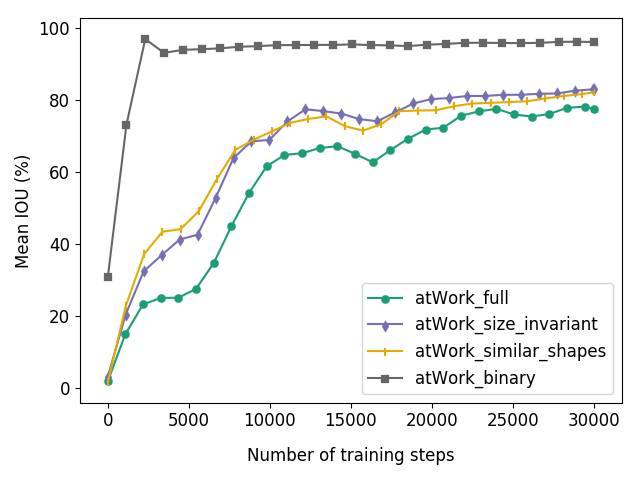
\includegraphics[width=1\linewidth]{images/mobi_4vars}
			%\label{Fig:mobivarsa}
		\end{subfigure}
		\begin{subfigure}{.5\textwidth}
			\centering
			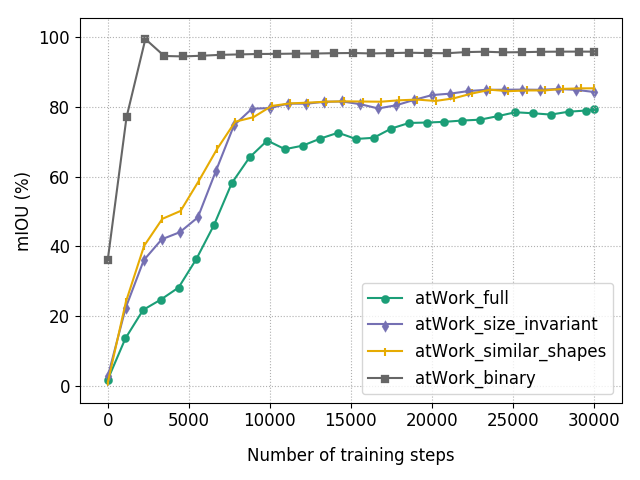
\includegraphics[width=1\linewidth]{images/mobi_4vars_white}
			%\label{Fig:mobivarsb}
		\end{subfigure}
		\caption{Mean IOU of deeplabv3+ with \textbf{mobileNet backbone} on variety of backgrounds dataset and white backgrounds dataset is shown. Mean IOU on the 4 variants of the variety of backgrounds dataset(left): atWork\_full = 77.47\%, atWork\_size\_invariant = 83.10\%, atWork\_similar\_shapes = 82.10\% and atWork\_binary = 96.06\%. Mean IOU on the 4 variants of the white backgrounds dataset(right): atWork\_full = 79.26\%, atWork\_size\_invariant = 84.29\%, atWork\_similar\_shapes = 85.33\% and atWork\_binary = 95.83\%.}
		\label{Fig:mobivars}
	\end{figure}
	
	\begin{figure}[!htb]
		\begin{subfigure}{.5\textwidth}
			\centering
			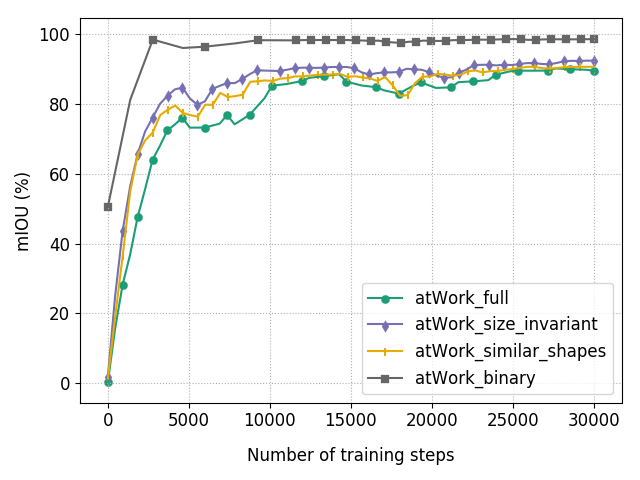
\includegraphics[width=1\linewidth]{images/xcep_4vars}
			%\label{Fig:mobivarsa}
		\end{subfigure}
		\begin{subfigure}{.5\textwidth}
			\centering
			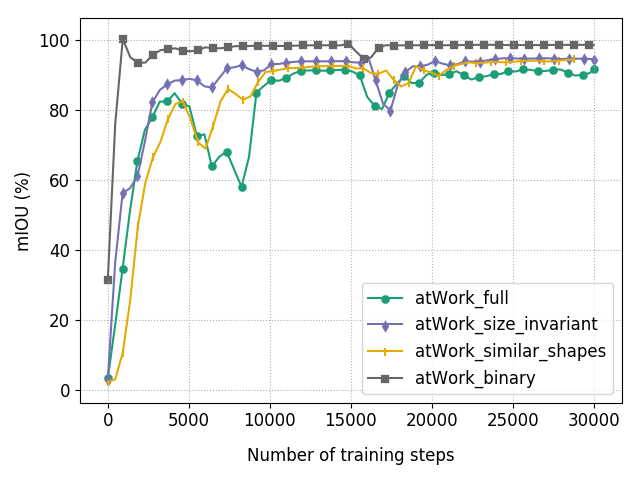
\includegraphics[width=1\linewidth]{images/xcep_4vars_white}
			%\label{Fig:mobivarsb}
		\end{subfigure}
		\caption{Mean IOU of deeplabv3+ with \textbf{xception backbone} on variety of backgrounds dataset and white backgrounds dataset is shown. Mean IOU on the 4 variants of the variety of backgrounds dataset(left): atWork\_full = 89.38\%, atWork\_size\_invariant = 91.19\%, atWork\_similar\_shapes = 90.81\% and atWork\_binary = 98.31\%. Mean IOU on the 4 variants of the white backgrounds dataset(right): atWork\_full = 91.59\%, atWork\_size\_invariant = 94.27\%, atWork\_similar\_shapes = 94.33\% and atWork\_binary = 98.47\%.}
		\label{Fig:xcepvars}
	\end{figure}
	
	\begin{figure}[!htb]
		\begin{subfigure}[c]{.5\textwidth}
			\centering
			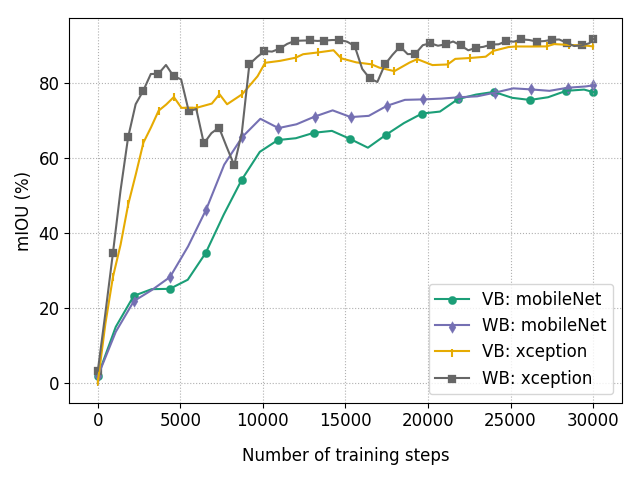
\includegraphics[width=1\linewidth]{images/mobxcep_full}
		\end{subfigure}
		\begin{subfigure}[c]{.5\textwidth}
			\centering
			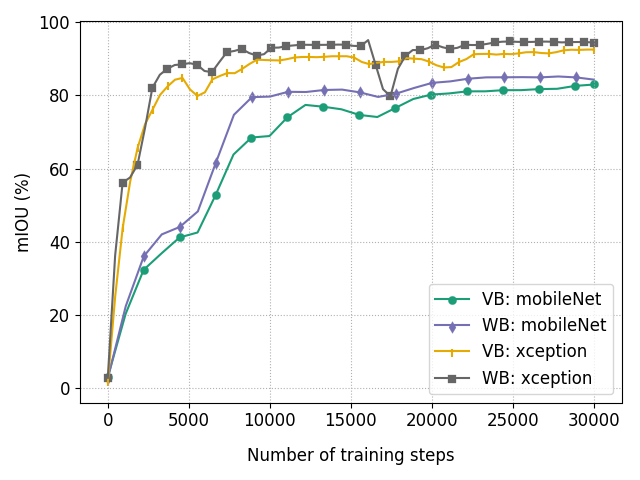
\includegraphics[width=1\linewidth]{images/mobxcep_size}
		\end{subfigure}
		\begin{subfigure}[c]{.5\textwidth}
			\centering
			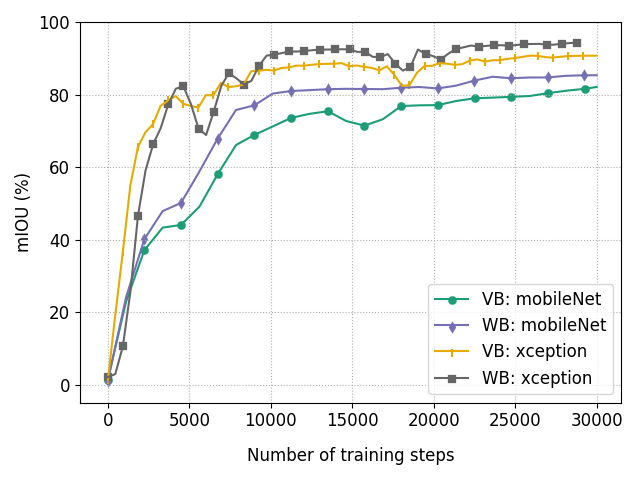
\includegraphics[width=1\linewidth]{images/mobxcep_shape}
		\end{subfigure}
		\begin{subfigure}[c]{.5\textwidth}
			\centering
			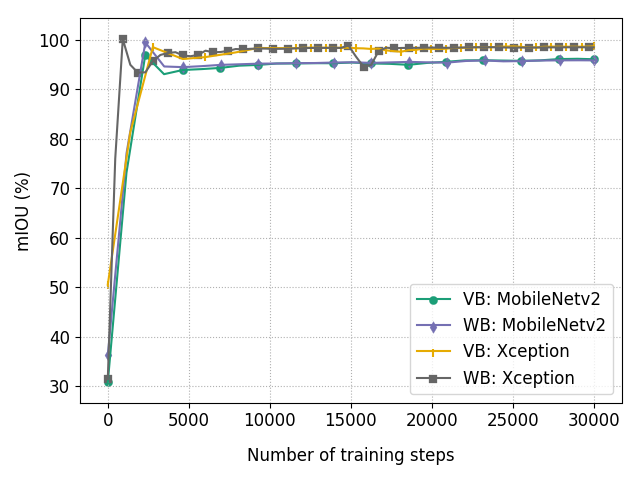
\includegraphics[width=1\linewidth]{images/mobxcep_binary}
		\end{subfigure}
		\caption{Comparision of Mean IOU obtained by deepLabv3+ using mobileNet backbone Vs xception backbone on all 4 variants. VB denotes variety of backgrounds dataset and WB denotes white backgrounds dataset. Top left: atWork\_full variant, top right: atWork\_size\_invariant, bottom left: atWork\_similar\_shapes and bottom left: atWork\_binary.}
		\label{Fig:4vars}
	\end{figure}

\subsection{Results on only the real validation set}

% both variety of backgrounds and white backgrounds

	\begin{figure}[!htb]
		\begin{subfigure}{.5\textwidth}
			\centering
			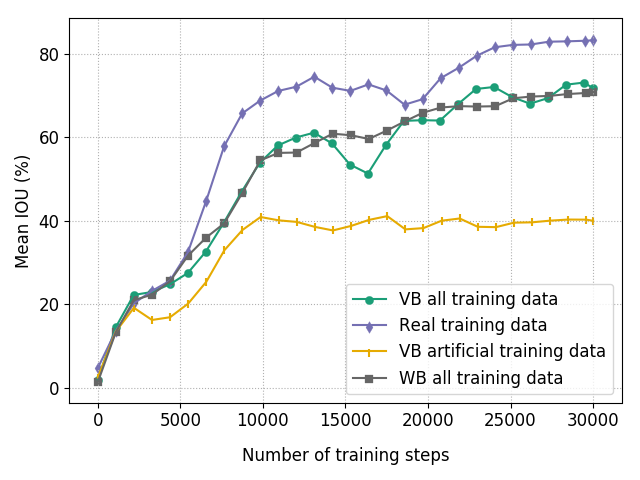
\includegraphics[width=1\linewidth]{images/re_val_mob_full}
		\end{subfigure}
		\begin{subfigure}{.5\textwidth}
			\centering
			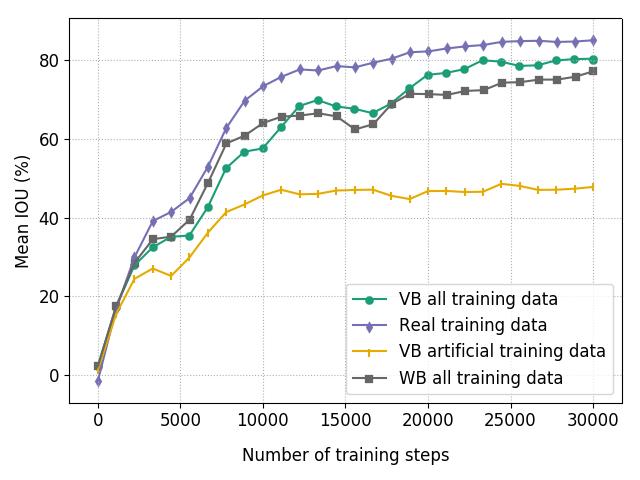
\includegraphics[width=1\linewidth]{images/re_val_mob_size}
		\end{subfigure}
		\begin{subfigure}{.5\textwidth}
			\centering
			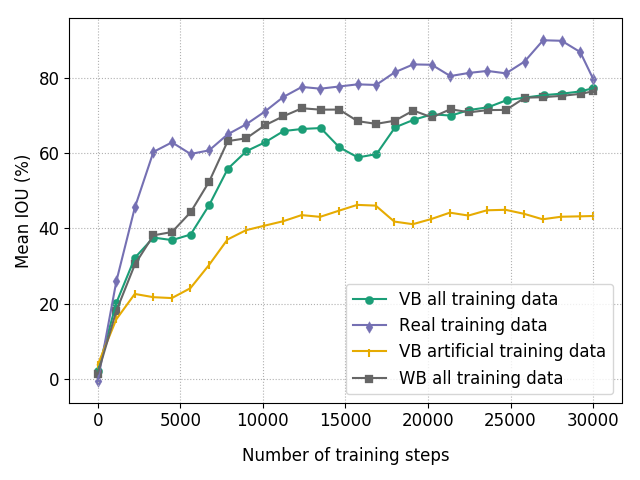
\includegraphics[width=1\linewidth]{images/re_val_mob_shape}
		\end{subfigure}
		\begin{subfigure}{.5\textwidth}
			\centering
			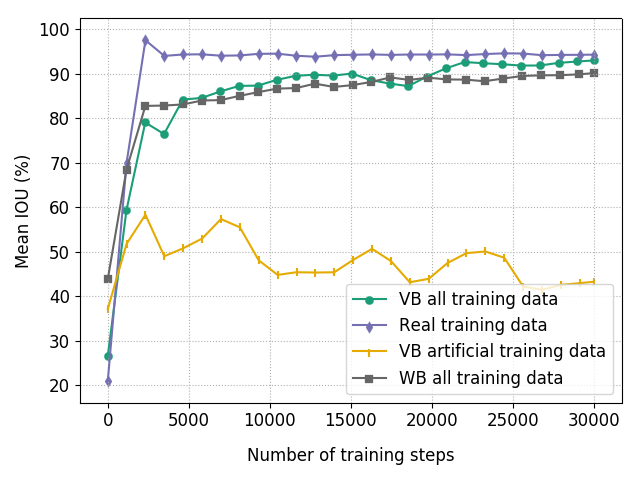
\includegraphics[width=1\linewidth]{images/re_val_mob_binary}
		\end{subfigure}
		\caption{Mean IOU on all 4 variants obtained by deepLabv3+ with mobileNet backbone when validated only on the real validation data. VB stands for variety of backgrounds dataset and WB stands for white backgrounds dataset. Top left: atWork\_full variant, top right: atWork\_size\_invariant, bottom left: atWork\_similar\_shapes and bottom left: atWork\_binary. The Mean IOUs are tabulated in \ref{Table:realval}}
		\label{Fig:realval}
	\end{figure}

\begin{table}[!htb]
	\centering
	\begin{tabular}{|c|c|c|c|c|c|c|c|}
	\hline 
    Variant & \makecell{Real \\training \\data} & \makecell{Variety\\ of backgrounds\\ all \\training data} & \makecell{White \\backgrounds\\ all \\training data} & \makecell{Variety\\ of backgrounds\\ artificial \\training data} \\ 
	\hline 
	atWork\_full & 83.21 & 71.72 & 70.8 & 40.0 \\ 
	\hline 
	atWork\_size\_invariant & 85.01 & 80.08 & 77.12 & 47.76 \\ 
	\hline 
	atWork\_similar\_shapes & 79.83 & 77.33 & 76.47 & 43.31 \\ 
	\hline 
	atWork\_binary & 94.33 & 93.01 & 90.17 & 43.29 \\ 
	\hline 
	\end{tabular}
	\caption{This table summarizes the results obtained when validating only on the real validation data. The first column denotes the variant. The remaining columns denote on what data was the deepLabv3+ with mobileNet backbone model trained on. All the Mean IOUs are in percentage.} 
	\label{Table:realval}
\end{table}

\subsection{Performance on individual classes}

% confusion matrix, histogram plots of class ious

	\begin{figure}[!htb]
		\begin{subfigure}[c]{1\textwidth}
			\centering
			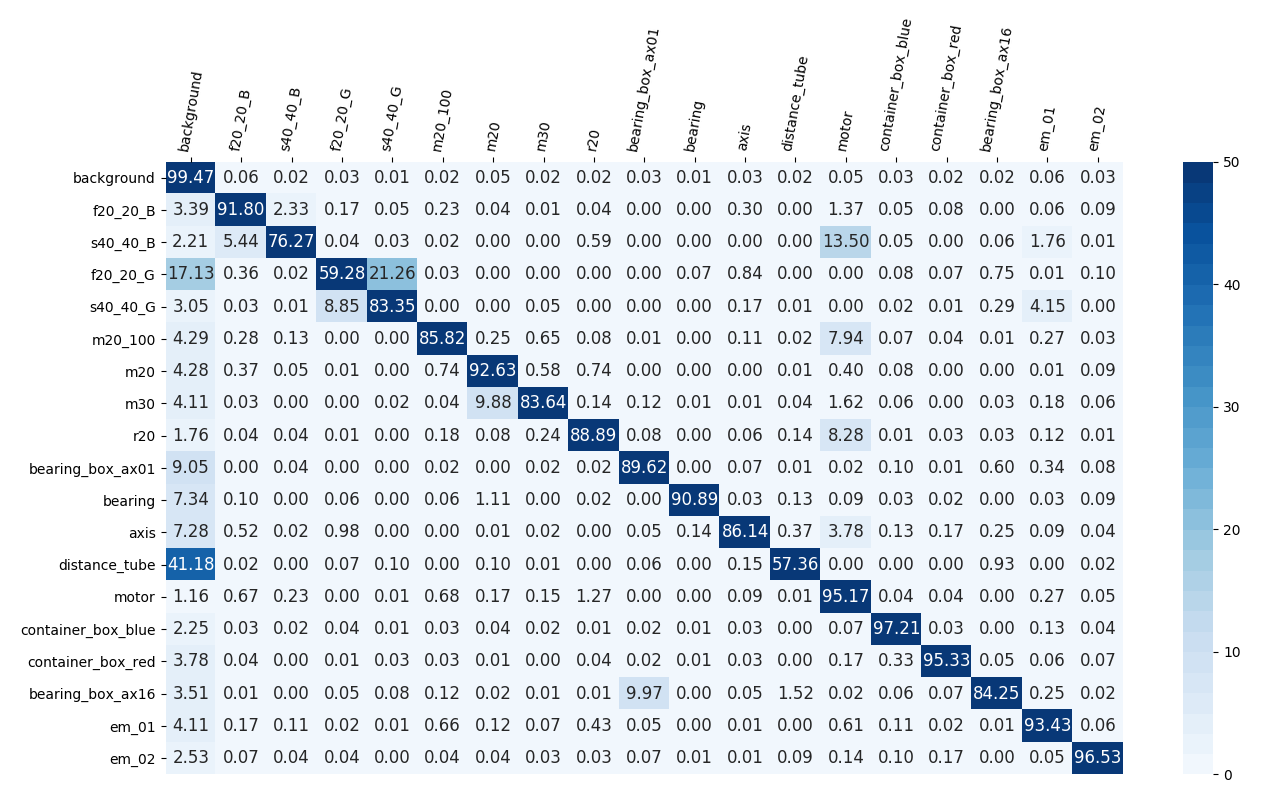
\includegraphics[width=1\linewidth]{images/cm_full}
		\end{subfigure}
		\begin{subfigure}[c]{.7\textwidth}
			\centering
			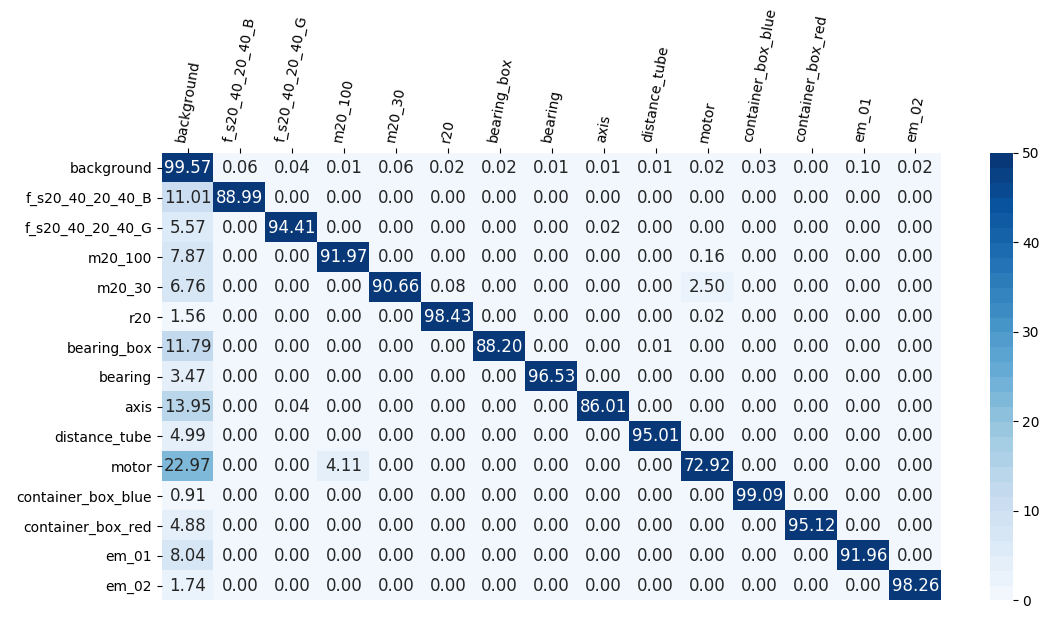
\includegraphics[width=1\linewidth]{images/cm_size}
		\end{subfigure}
		\begin{subfigure}[c]{.6\textwidth}
			\centering
			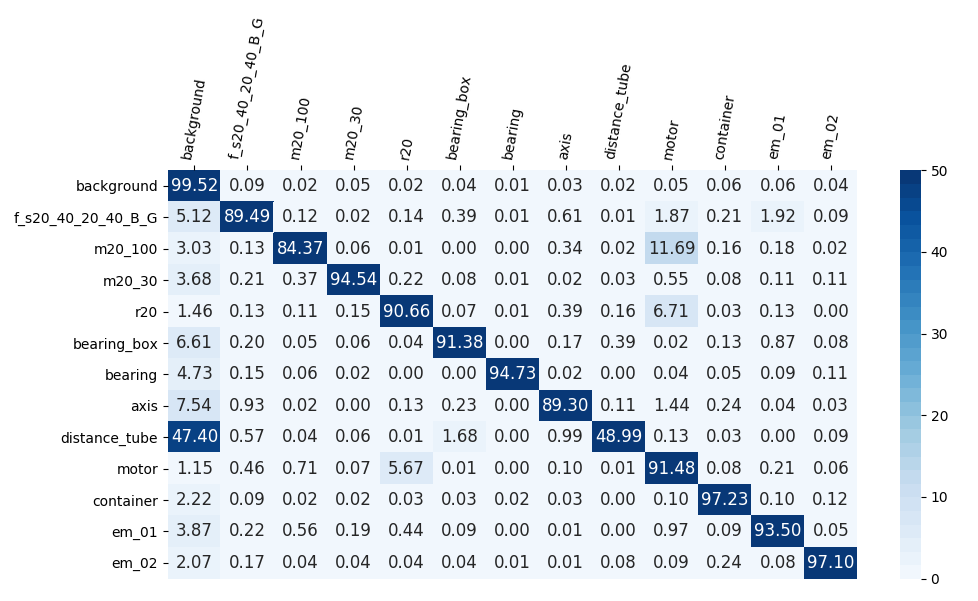
\includegraphics[width=1\linewidth]{images/cm_shape}
		\end{subfigure}
		\begin{subfigure}[c]{.3\textwidth}
			\centering
			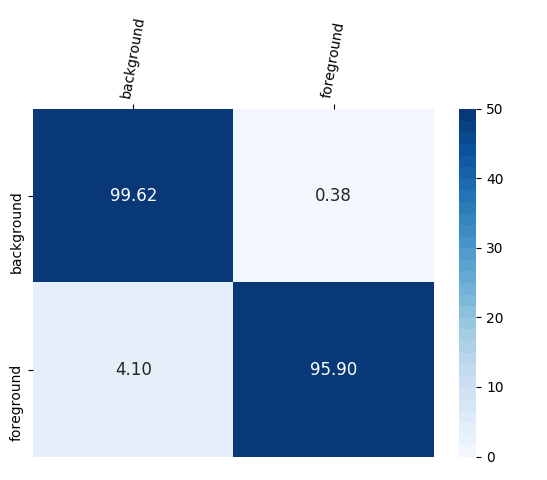
\includegraphics[width=1\linewidth]{images/cm_binary}
		\end{subfigure}
		\caption{Confusion matrix based on number of classified pixels on all 4 variants of the variety of backgrounds dataset. The number of pixels in each row is normalized by the total number of pixels in the row. First row: atWork\_full variant, second row: atWork\_size\_invariant, third row left: atWork\_similar\_shapes and third row left: atWork\_binary.}
		\label{Fig:cm}
	\end{figure}
	
	\begin{figure}[!htb]
		\begin{subfigure}{1\textwidth}
			\centering
			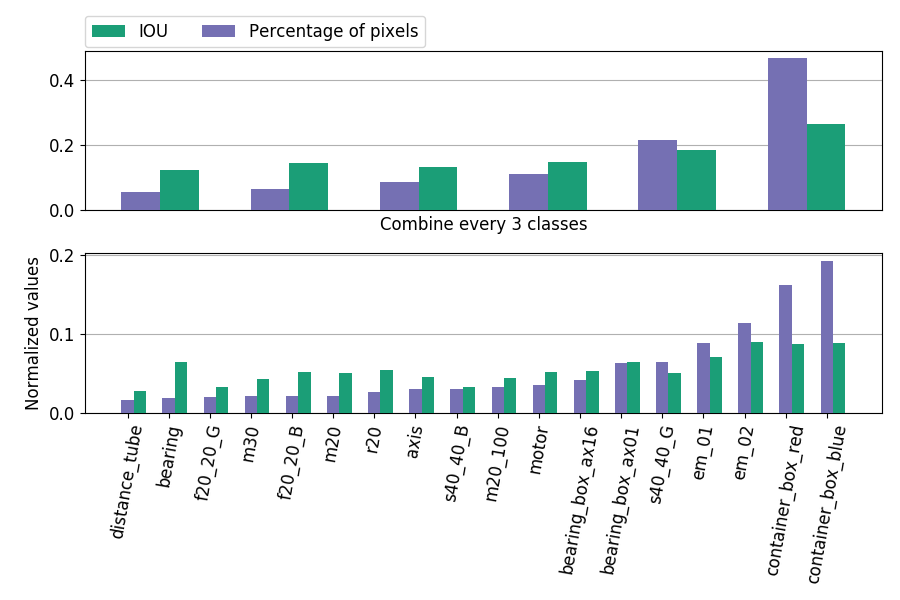
\includegraphics[width=1\linewidth]{images/cls_iou_full}
		\end{subfigure}
		\begin{subfigure}{.5\textwidth}
			\centering
			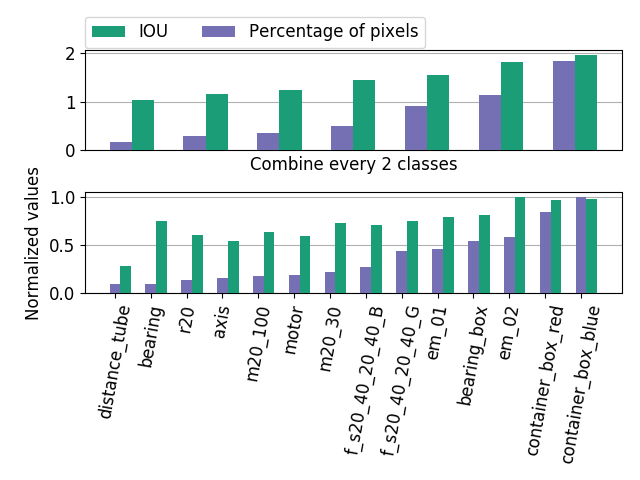
\includegraphics[width=1\linewidth]{images/cls_iou_size}
		\end{subfigure}
		\begin{subfigure}{.5\textwidth}
			\centering
			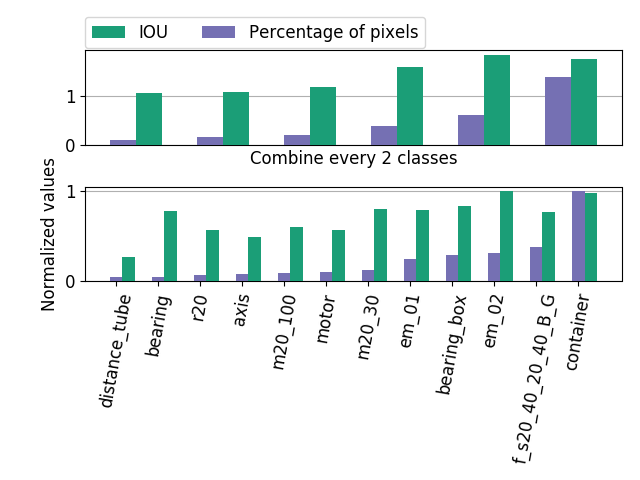
\includegraphics[width=1\linewidth]{images/cls_iou_shape}
		\end{subfigure}
		\caption{Individual class IOUs plotted with the percentage of pixels occupied on all 4 variants of the variety of backgrounds dataset. The number of pixels in each row is normalized by the total number of pixels in the row. Top left: atWork\_full variant, top right: atWork\_size\_invariant, bottom left atWork\_similar\_shapes and bottom left atWork\_binary.}
		\label{Fig:clsiou}
	\end{figure}

\subsection{Learning rate}

	\begin{figure}[!htb]
		\begin{subfigure}{.3\textwidth}
			\centering
			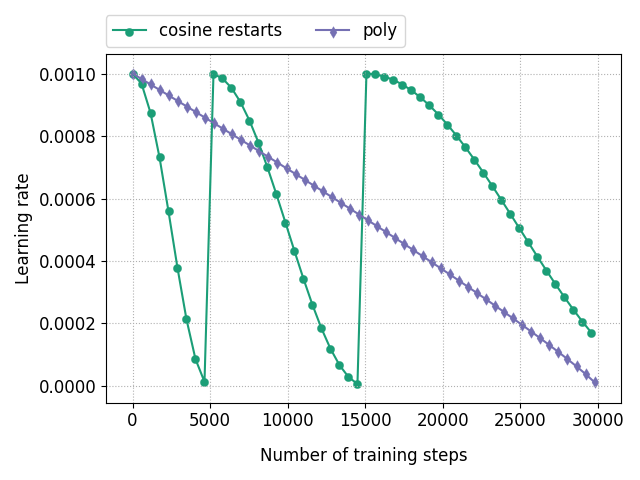
\includegraphics[width=1\linewidth]{images/lr_train_bin}
		\end{subfigure}
		\begin{subfigure}{.3\textwidth}
			\centering
			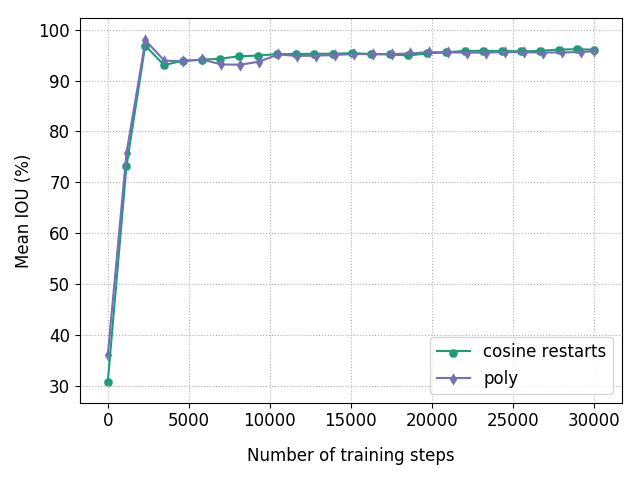
\includegraphics[width=1\linewidth]{images/lr_binary}
		\end{subfigure}
		\begin{subfigure}{.3\textwidth}
			\centering
			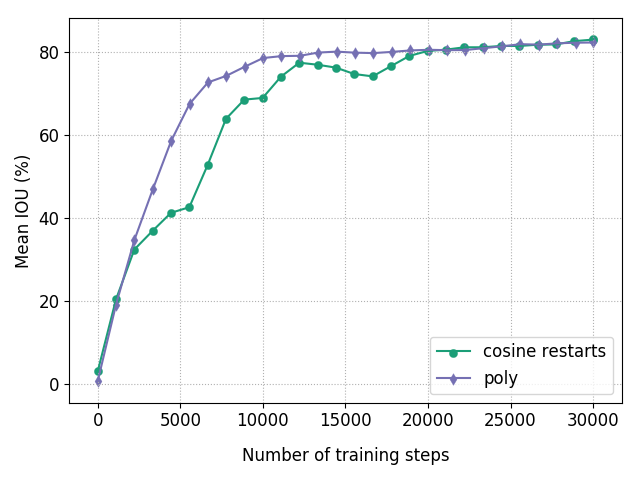
\includegraphics[width=1\linewidth]{images/lr_size}
		\end{subfigure}
		\caption{Learning rate decay with two different policies 1. cosine restarts and 2. poly is compared. Left: learning rate over 30000 steps with the two decay policies. Middle: Mean IOU on the validation set of atWork\_binary variant is 96.06 \% with cosine restarts and 95.75 \% with poly. Right: Mean IOU on the validation set of atWork\_size\_invariant variant is 83.1 \% with cosine restarts and 82.24 \% with poly.}
		\label{Fig:lr}
	\end{figure}

\subsection{Class balancing}

% About attempt to counter failure in distance tube.

\subsection{Performance of quantized models}

	\begin{figure}[!htb]
		\begin{subfigure}{.5\textwidth}
			\centering
			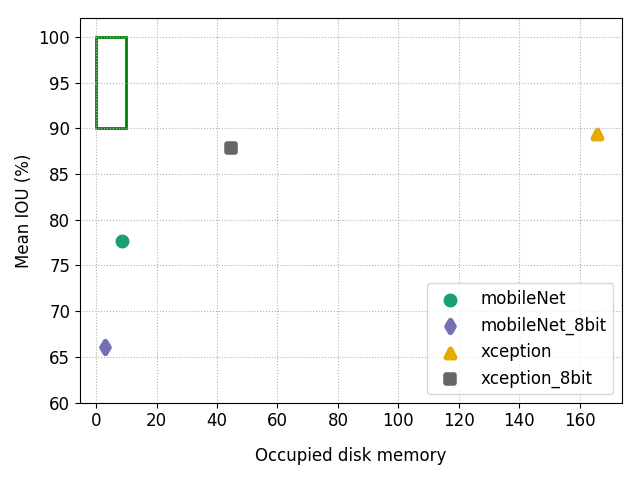
\includegraphics[width=1\linewidth]{images/q_mem_v_full}
		\end{subfigure}
		\begin{subfigure}{.5\textwidth}
			\centering
			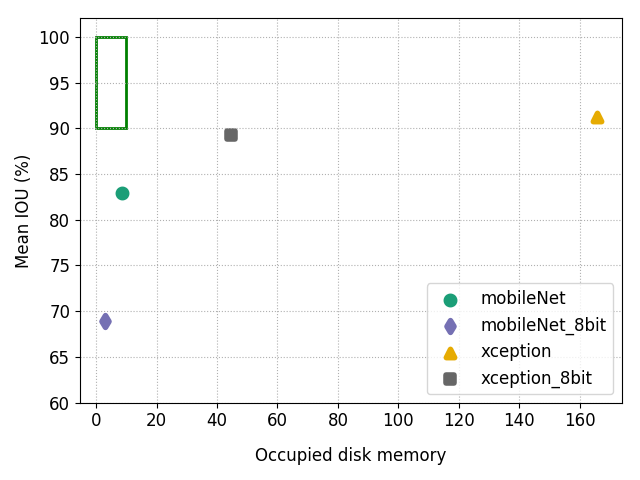
\includegraphics[width=1\linewidth]{images/q_mem_v_size}
		\end{subfigure}
		\begin{subfigure}{.5\textwidth}
			\centering
			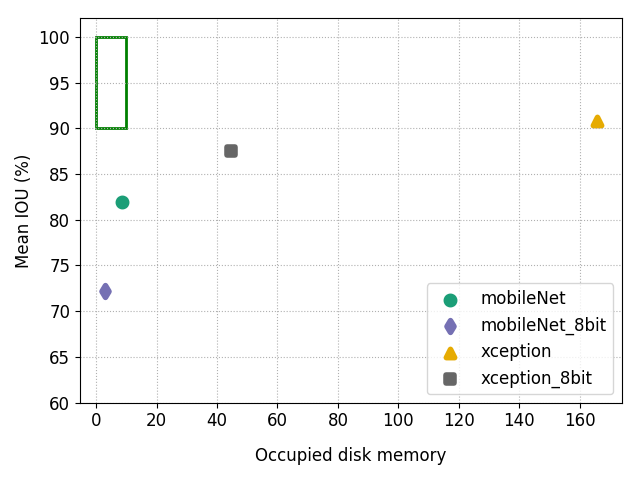
\includegraphics[width=1\linewidth]{images/q_mem_v_shape}
		\end{subfigure}
		\begin{subfigure}{.5\textwidth}
			\centering
			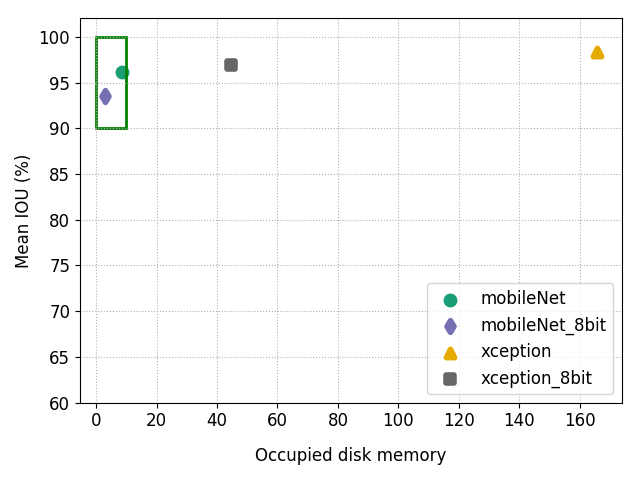
\includegraphics[width=1\linewidth]{images/q_mem_v_bin}
		\end{subfigure}
		\caption{.}
		\label{Fig:quant}
	\end{figure}

\subsection{Transfer learning}

\begin{figure}[htb!]
	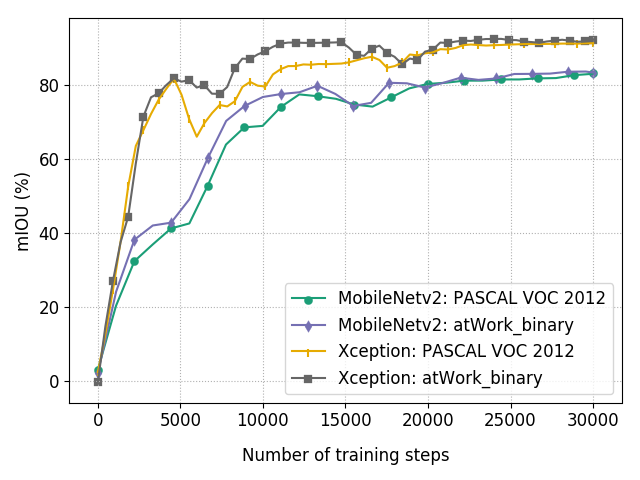
\includegraphics[scale=0.4]{images/transfer_size}
	\caption{Size invariant;mobileNet: PASCAL VOC 2012 = 83.1, mobileNet: atWork\_binary = 83.26, xception: PASCAL VOC 2012 = 91.19, xception: atWork\_binary = 92.14}
\end{figure}

\begin{figure}[htb!]
	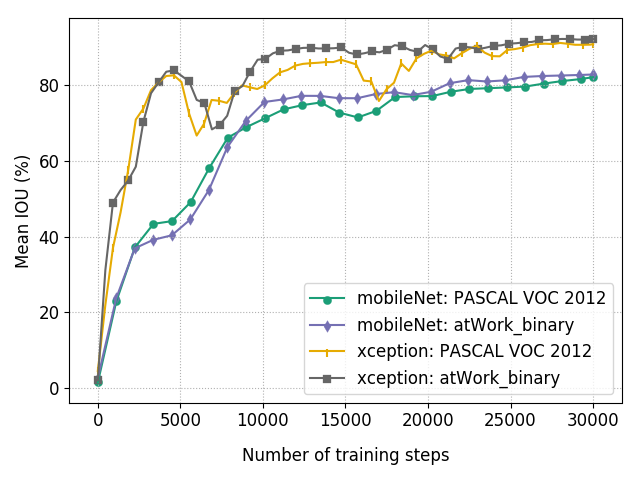
\includegraphics[scale=0.4]{images/transfer_shape}
	\caption{Similar shapes;mobileNet: PASCAL VOC 2012 = 82.1, mobileNet: atWork\_binary = 82.8, xception: PASCAL VOC 2012 = 90.81, xception: atWork\_binary = 92.15}
\end{figure}

\begin{figure}[htb!]
	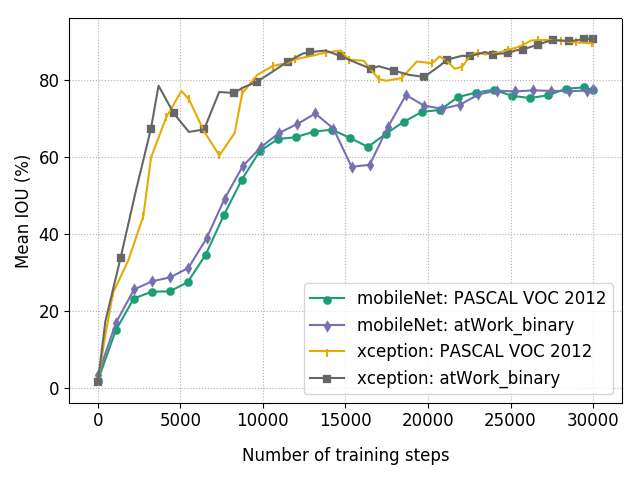
\includegraphics[scale=0.4]{images/transfer_full}
	\caption{Full;mobileNet: PASCAL VOC 2012 = 77.47, mobileNet: atWork\_binary = 77.73, xception: PASCAL VOC 2012 = 89.38, xception: atWork\_binary = 90.64}
\end{figure}

